\documentclass[]{article}
\usepackage{lmodern}
\usepackage{amssymb,amsmath}
\usepackage{ifxetex,ifluatex}
\usepackage{fixltx2e} % provides \textsubscript
\ifnum 0\ifxetex 1\fi\ifluatex 1\fi=0 % if pdftex
  \usepackage[T1]{fontenc}
  \usepackage[utf8]{inputenc}
\else % if luatex or xelatex
  \ifxetex
    \usepackage{mathspec}
    \usepackage{xltxtra,xunicode}
  \else
    \usepackage{fontspec}
  \fi
  \defaultfontfeatures{Mapping=tex-text,Scale=MatchLowercase}
  \newcommand{\euro}{€}
\fi
% use upquote if available, for straight quotes in verbatim environments
\IfFileExists{upquote.sty}{\usepackage{upquote}}{}
% use microtype if available
\IfFileExists{microtype.sty}{%
\usepackage{microtype}
\UseMicrotypeSet[protrusion]{basicmath} % disable protrusion for tt fonts
}{}
\usepackage[margin=1in]{geometry}
\usepackage{color}
\usepackage{fancyvrb}
\newcommand{\VerbBar}{|}
\newcommand{\VERB}{\Verb[commandchars=\\\{\}]}
\DefineVerbatimEnvironment{Highlighting}{Verbatim}{commandchars=\\\{\}}
% Add ',fontsize=\small' for more characters per line
\usepackage{framed}
\definecolor{shadecolor}{RGB}{248,248,248}
\newenvironment{Shaded}{\begin{snugshade}}{\end{snugshade}}
\newcommand{\KeywordTok}[1]{\textcolor[rgb]{0.13,0.29,0.53}{\textbf{{#1}}}}
\newcommand{\DataTypeTok}[1]{\textcolor[rgb]{0.13,0.29,0.53}{{#1}}}
\newcommand{\DecValTok}[1]{\textcolor[rgb]{0.00,0.00,0.81}{{#1}}}
\newcommand{\BaseNTok}[1]{\textcolor[rgb]{0.00,0.00,0.81}{{#1}}}
\newcommand{\FloatTok}[1]{\textcolor[rgb]{0.00,0.00,0.81}{{#1}}}
\newcommand{\CharTok}[1]{\textcolor[rgb]{0.31,0.60,0.02}{{#1}}}
\newcommand{\StringTok}[1]{\textcolor[rgb]{0.31,0.60,0.02}{{#1}}}
\newcommand{\CommentTok}[1]{\textcolor[rgb]{0.56,0.35,0.01}{\textit{{#1}}}}
\newcommand{\OtherTok}[1]{\textcolor[rgb]{0.56,0.35,0.01}{{#1}}}
\newcommand{\AlertTok}[1]{\textcolor[rgb]{0.94,0.16,0.16}{{#1}}}
\newcommand{\FunctionTok}[1]{\textcolor[rgb]{0.00,0.00,0.00}{{#1}}}
\newcommand{\RegionMarkerTok}[1]{{#1}}
\newcommand{\ErrorTok}[1]{\textbf{{#1}}}
\newcommand{\NormalTok}[1]{{#1}}
\usepackage{graphicx}
\makeatletter
\def\maxwidth{\ifdim\Gin@nat@width>\linewidth\linewidth\else\Gin@nat@width\fi}
\def\maxheight{\ifdim\Gin@nat@height>\textheight\textheight\else\Gin@nat@height\fi}
\makeatother
% Scale images if necessary, so that they will not overflow the page
% margins by default, and it is still possible to overwrite the defaults
% using explicit options in \includegraphics[width, height, ...]{}
\setkeys{Gin}{width=\maxwidth,height=\maxheight,keepaspectratio}
\ifxetex
  \usepackage[setpagesize=false, % page size defined by xetex
              unicode=false, % unicode breaks when used with xetex
              xetex]{hyperref}
\else
  \usepackage[unicode=true]{hyperref}
\fi
\hypersetup{breaklinks=true,
            bookmarks=true,
            pdfauthor={Andresa de Andrade},
            pdftitle={Central limit theorem and Convergence},
            colorlinks=true,
            citecolor=blue,
            urlcolor=blue,
            linkcolor=magenta,
            pdfborder={0 0 0}}
\urlstyle{same}  % don't use monospace font for urls
\setlength{\parindent}{0pt}
\setlength{\parskip}{6pt plus 2pt minus 1pt}
\setlength{\emergencystretch}{3em}  % prevent overfull lines
\setcounter{secnumdepth}{5}

%%% Use protect on footnotes to avoid problems with footnotes in titles
\let\rmarkdownfootnote\footnote%
\def\footnote{\protect\rmarkdownfootnote}

%%% Change title format to be more compact
\usepackage{titling}
\setlength{\droptitle}{-2em}
  \title{Central limit theorem and Convergence}
  \pretitle{\vspace{\droptitle}\centering\huge}
  \posttitle{\par}
  \author{Andresa de Andrade}
  \preauthor{\centering\large\emph}
  \postauthor{\par}
  \predate{\centering\large\emph}
  \postdate{\par}
  \date{July 2, 2014}




\begin{document}

\maketitle


{
\hypersetup{linkcolor=black}
\setcounter{tocdepth}{2}
\tableofcontents
}
\hyperdef{}{toc}{}
\newpage 

\section{Exponential Distribuition}\label{exponential-distribuition}

Simulating a exponential variable with lambda 0.2 and k = 10000

\begin{Shaded}
\begin{Highlighting}[]
\NormalTok{n=}\StringTok{ }\DecValTok{40}
\NormalTok{lambda =}\StringTok{ }\FloatTok{0.2}
\NormalTok{k=}\DecValTok{10000}
\NormalTok{list_of_exponential =}\StringTok{ }\KeywordTok{array}\NormalTok{(}\DecValTok{1}\NormalTok{:k)}

\NormalTok{for(i in }\DecValTok{1}\NormalTok{:k)\{}
  \NormalTok{list_of_exponential[i] =}\StringTok{ }\KeywordTok{mean}\NormalTok{(}\KeywordTok{rexp}\NormalTok{(n, lambda))}
\NormalTok{\}}
\end{Highlighting}
\end{Shaded}

Let's calculate where the distribution of the mean when it's centered
and compare to the theoretical center

\begin{Shaded}
\begin{Highlighting}[]
\NormalTok{mean_of_average =}\StringTok{ }\KeywordTok{mean}\NormalTok{(list_of_exponential)}
\NormalTok{mean_of_average}
\end{Highlighting}
\end{Shaded}

\begin{verbatim}
## [1] 5.009134
\end{verbatim}

Meanwhile, the expected value for mean is 1/lambda = 5.

\begin{Shaded}
\begin{Highlighting}[]
\NormalTok{sd_mean =}\StringTok{ }\KeywordTok{sd}\NormalTok{(list_of_exponential)}
\NormalTok{sd_mean}
\end{Highlighting}
\end{Shaded}

\begin{verbatim}
## [1] 0.7948422
\end{verbatim}

The expected Standard Deviation is
\{{[}1/(lambda)\^{}(2){]}/n\}\^{}(0.5)

\begin{verbatim}
## [1] 0.7905694
\end{verbatim}

1- When we compare the theoretical center we were expecting the average
to be 5. it's 5.07.

2- And we were expecting the standard deviation to 0.79 and it's 0.784.

3-For the approximation to a normal, we can check the figure 1 in the
appendix. the curve is a normal(5,0.7906) and the histogram is referent
to the the mean distribution. We can see that it clearly looks like a
normal. To understand how well fitted is the model I have generate 1000
normal variables (Figure 2) as if I wanted to check how they look like,
and they are as good as the exponential distribution (even better in my
opinion). So we can conclude that when n increases, the exponential
converges to a normal.

4- As 1/lambda is the mean for this distribution we have that at 95\% of
confidence the mean is in this interval:

\begin{verbatim}
## [1] 4.993555 5.024713
\end{verbatim}

\section{Conclusion}\label{conclusion}

From the points above we can conclude that the hypothesis of convergence
is consistent for exponential distribution and the mean of n exponential
converges to the distribution mean.

\newpage

\section{Appendix}\label{appendix}

\begin{figure}[htbp]
\centering
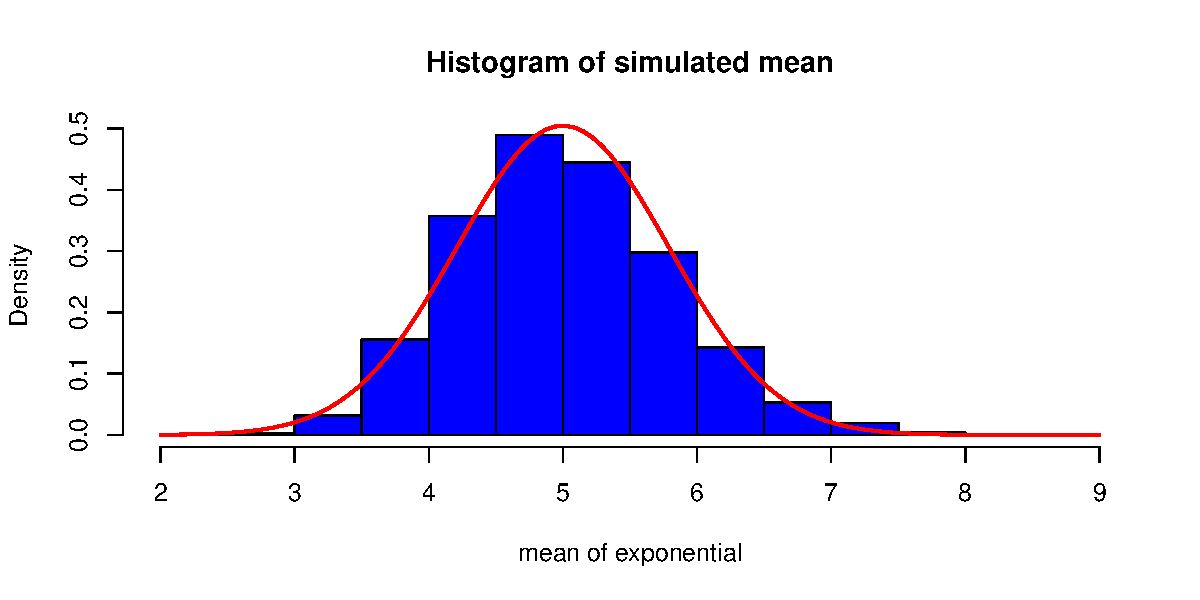
\includegraphics{TCL_Convergence_files/figure-latex/unnamed-chunk-6-1.pdf}
\caption{Histogram of Simulated Mean}
\end{figure}

\begin{figure}[htbp]
\centering
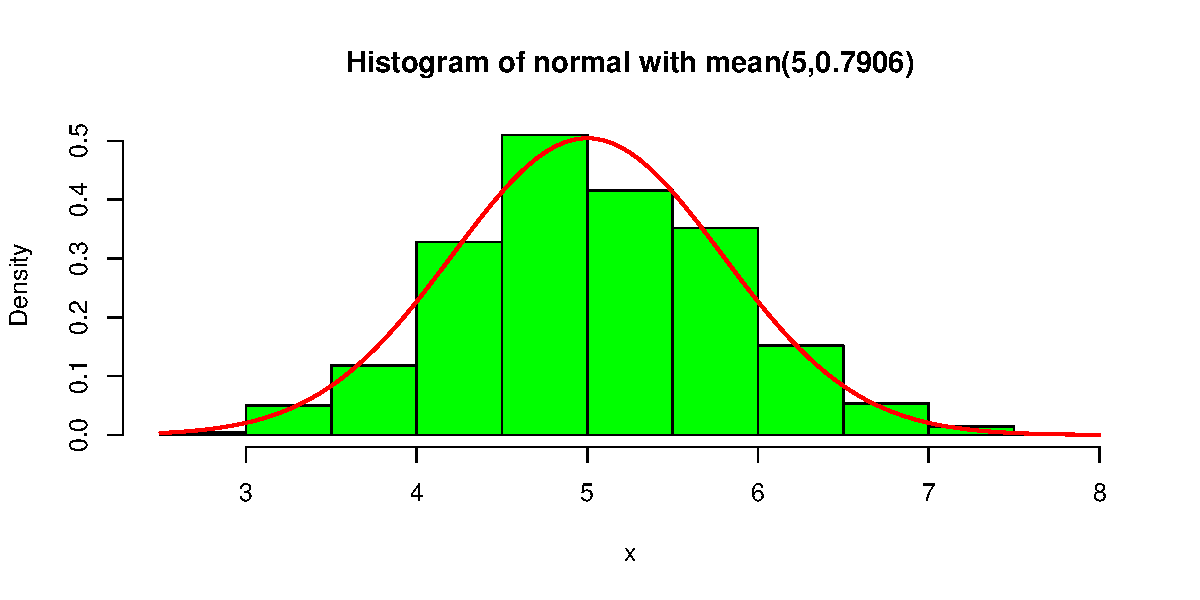
\includegraphics{TCL_Convergence_files/figure-latex/unnamed-chunk-7-1.pdf}
\caption{Histogram ofg a Normal distribution.}
\end{figure}

\end{document}
